\chapter{Objetivos}
\label{cap:capitulo2}

\begin{flushright}
\begin{minipage}[]{10cm}
\emph{Dame seis horas para talar un árbol y pasaré las primeras cuatro afilando el hacha}\\
\end{minipage}\\

Abraham Licoln\\
\end{flushright}

\vspace{1cm}

Una vez establecido el marco contextual de este proyecto, se procederá a
presentar una descripción del problema a abordar, así como el proceso creativo e
intelectual que guiará el desarrollo del mismo, lo que incluirá los requisitos
del proyecto, la metodología empleada y el plan de trabajo detallado.

%Escribe aquí un párrafo explicando brevemente lo que vas a contar en este capítulo. En este capítulo lo ideal es explicar cuáles han sido los objetivos que te has fijado conseguir con tu trabajo, qué requisitos ha de respetar el resultado final, y cómo lo has llevado a cabo; esto es, cuál ha sido tu plan de trabajo.\\

\section{Descripción del problema}
\label{sec:descripcion}

Este proyecto surge como respuesta a la escasa investigación acerca del
paradigma de programación de flujos de datos empleados en conjunto con ROS2,
ofreciendo a su vez un entorno propicio para la creación sencilla de distintas
aplicaciones robóticas basadas en dichos flujos de datos, que pueden replicar de
manera versátil y sencilla los comportamientos reactivos de los robots,
eludiendo la complejidad inherente de este \textit{middleware} robótico (ROS2) y
dando lugar, por tanto, a un nuevo entorno de programación más simple, a la vez
que solucionando varios problemas expuestos a continuación.


\subsection{El problema de la congestión de red}
\label{sec:problema_congestion}

Con el uso de ROS2, que por defecto funciona sobre el protocolo DDS, existe un
problema de congestión de red: los nodos de ROS2 generan una gran cantidad de
mensajes de manera iterativa, que a su vez se transmiten a través de DDS, siendo
este un protocolo de comunicaciones que, por su naturaleza, origina muchos de
mensajes de \textit{Discovery}, lo que en conjunto conlleva a la congestión de
la red, y dificulta de esta manera la programación de aplicaciones multirobot.
\\

Una solución muy sencilla a este problema consistirá en cambiar el protocolo que
lo provoca por otro con mejores prestaciones.
En nuestro caso se utilizará un protocolo llamado Zenoh, como ya se expondrá más
adelante, en el Capítulo \ref{cap:capitulo3}.


\subsection{El problema del escalón de aprendizaje en robótica}
\label{sec:problema_escalon}

La educación en robótica se basa principalmente en robots de bajo coste, como se
expuso en la Sección \ref{sec:robotica_educativa}, lo que suele limitar la
capacidad del robot en cuestión y merma la cantidad de \textit{hardware} externo
compatible, así como su calidad, y consecuentemente limita la creatividad y el
aprendizaje de los estudiantes.
Además, siendo ROS el estándar en robótica para la programación de robots,
se genera un escalón de aprendizaje, previamente expuesto en la sección
referenciada, debido al gran cambio desde la programación de placas como
Arduino, a la utilización tanto de \textit{hardware}, como de \textit{software}
mucho más complejos.
\\

Esto conlleva a una gran diferencia entre la robótica que se enseña en las
etapas de la educación primaria y secundaria respecto a la etapa universitaria,
y es debido precisamente, a la complejidad de código y enseñanza de ROS, para
los cuales, se requiere incluso de varias asignaturas en esta última etapa.
Es por este motivo, que este trabajo pretende incorporar un paso intermedio en
la enseñanza, simplificando el desarrollo del  \textit{software} en ROS2, y
dando la posibilidad de crear aplicaciones robóticas más complejas de una manera
más simple para robots más completos, y que a su vez permanecen dentro de la
categoría de robots de bajo coste, siendo asequibles para instituciones como
colegios o institutos.


\subsection{Planteamiento de la solución}
\label{sec:planteamiento_solucion}

La simplicidad del código de ROS2 se conseguirá gracias al uso de un
\textit{framework} llamado Zenoh-Flow, que funciona sobre el protocolo
mencionado en la Sección \ref{sec:problema_congestion}, y el cuál le da
nombre.
Este \textit{framework} está pensado para la programación de flujos de datos,
por lo que se requerirá la previa definición de un flujo de datos a seguir por
parte de los nodos, los cuales activarán su iteración al momento de recibir un
dato, y generarán ---en su conjunto--- un flujo de datos transmitiendo los datos
de nodo a nodo únicamente cuando es necesario, cualidad que reducirá en gran
cantidad los mensajes generados.
\\

La implementación conjunta con ROS2 será posible gracias a que Zenoh-Flow
permite serializar los datos que se quieren enviar, y existe un \textit{bridge}
que los traduce de Zenoh a DDS y viceversa, para que los nodos de ROS2 y de
Zenoh-Flow puedan entender la información que se envían.
Es por este motivo que se serializarán los mensajes de la misma manera que se
hace internamente en ROS2, y así se podrá seguir utilizando nodos de ROS2
existentes, como pueden ser los relativos a la navegación, lo que evitará la
complejidad de su programación.
\\

Este trabajo pretende, por tanto, solucionar el problema del escalón de
aprendizaje, suponiendo un paso intermedio en la enseñanza de la robótica, así
como el problema de la congestión de red generada por DDS, suponiendo una
posible solución a la misma, además de presentar una entorno en el que se puede
aplicar el paradigma de programación de flujos de datos en conjunto con ROS2.
\\

Con el fin de resolver estos problemas, y cumplir los objetivos principales
descritos, se detallan a continuación los siguientes subobjetivos:

\begin{enumerate}
    \item{Desarrollo de un entorno de programación que posibilite la
        programación de flujos de datos.}
    \item{La solución anterior debe ser funcional en conjunto con nodos de ROS2,
        permitiendo la mutua comunicación entre ambos \textit{softwares} de
        manera bidireccional.}
    \item{El desarrollo de una aplicación robótica en simulación utilizando el
        anterior entorno de desarrollo de flujos de datos.}
    \item{El traslado de la anterior aplicación a un entorno con robots reales.}
    \item{Demostrar la simplicidad de código y la viabilidad de su aplicación en
        entornos educativos, solventando el escalón de aprendizaje descrito.}
    \item{Disminuir la congestión de red originada por DDS.}
\end{enumerate}

%Cuenta aquí el objetivo u objetivos generales y, a continuación, concrétalos mediante objetivos específicos.

\section{Requisitos}
\label{sec:requisitos}

Para solucionar los problemas descritos, además de cumplir los subobjetivos
marcados, este trabajo deberá cumplir los siguientes requisitos:

\begin{enumerate}
    \item{Se utilizará \textit{GNU/Linux}, con la distribución
        \textit{Ubuntu 22.04 LTS} como sistema operativo en todos los
        \textit{hardwares}.}
    \item{Las herramientas \textit{software} utilizadas deben ser compatibles
        para funcionar correctamente en conjunto.}
    \item{Las aplicaciones demostrativas que se desarrollen deben ser fácilmente
        reproducibles y desplegables tanto en un entorno simulado como en un
        ambiente educativo real o de laboratorio.}
    \item{El desarrollo del \textit{software} debe ser lo suficientemente
        sencillo para poder ser llevado a cabo por alumnos preuniversitarios.}
    \item{El \textit{hardware} utilizado debe ser suficientemente económico para
        ser adquirido por cualquier institución educativa, independientemente
        del presupuesto del que dispongan.}
\end{enumerate}



\section{Competencias}
\label{sec:requisitos}

Las competencias generales que se cumplen con la realización de este trabajo de
fin de grado, según la guía docente de la asignatura, son las siguientes:

\begin{enumerate}
    \item{\textit{CB2.} Que los estudiantes sepan aplicar sus conocimientos a su
        trabajo o vocación de una forma profesional y posean las competencias
        que suelen demostrarse por medio de la elaboración y defensa de
        argumentos y la resolución de problemas dentro de su área de estudio.}
        Esta competencia se cumple con la realización de la parte del
        \textit{software} de este trabajo, en la que se aplican distintos
        conocimientos adquiridos durante el grado.
    \item{\textit{CB4.} Que los estudiantes puedan transmitir información,
        ideas, problemas y soluciones a un público tanto especializado como no
        especializado.}
        Esta competencia se adquiere al detallar todo el complejo proceso
        consecuente a este trabajo de manera clara y comprensible en el presente
        documento.
    \item{\textit{CB5.} Que los estudiantes hayan desarrollado aquellas
        habilidades de aprendizaje necesarias para emprender estudios
        posteriores con un alto grado de autonomía.}
        Esta competencia queda cumplida al adquirir los conocimientos
        suficientes para el desarrollo de este trabajo de manera completamente
        autónoma, a base de distintas pruebas y consultas en distintas fuentes:
        publicaciones científicas, foros de desarrollo en la web, etc.
\end{enumerate}

La competencia específica \textit{CE28} de la asignatura detalla lo
siguiente:
Desarrollo de las capacidades adecuadas para realizar un ejercicio original
individual (o excepcionalmente colectivo), presentarlo y defenderlo ante un
tribunal universitario, consistente en un proyecto en el ámbito de las
tecnologías específicas del campo de la Robótica de naturaleza profesional en el
que se sinteticen e integren las competencias adquiridas en las enseñanzas.
Esta última competencia se cumple con el desarrollo de este proyecto, la
investigación  del estado del arte en el que se enmarca, la confección de su
memoria, y su defensa ante un tribunal.

%Describe los requisitos que ha de cumplir tu trabajo.

\section{Metodología}
\label{sec:metodologia}

La metodología utilizada sigue pautas de investigación sobre el estado del arte
previo al trabajo, y posteriormente sobre el \textit{software} utilizado,
siempre evaluando de antemano la compatibilidad con el \textit{hardware}
disponible, así como realizando pruebas pertinentes sobre su correcto
funcionamiento en los distintos entornos, incluyendo la simulación y el
laboratorio.
\\

En relación con el desarrollo del \textit{software} demostrativo se siguió un
ciclo de desarrollo \textit{software} iterativo, que consiste en la
planificación del \textit{software}, el desarrollo del mismo, su consecuente
revisión mediante pruebas y su corrección, todo ello de manera periódica,
generando en cada una de las iteraciones un resultado ejecutable mejor que el
anterior, hasta conseguir al final una versión completamente funcional, como se
ve reflejado en la Figura \ref{fig:desarrollo_iterativo}.
Este proceso de desarrollo puede verse alineado con los principios de mejora
continua del ciclo de desarrollo PDCA (\textit{Plan}, \textit{Do},
\textit{Check}, \textit{Act}).
\\

\begin{figure} [h!]
  \begin{center}
    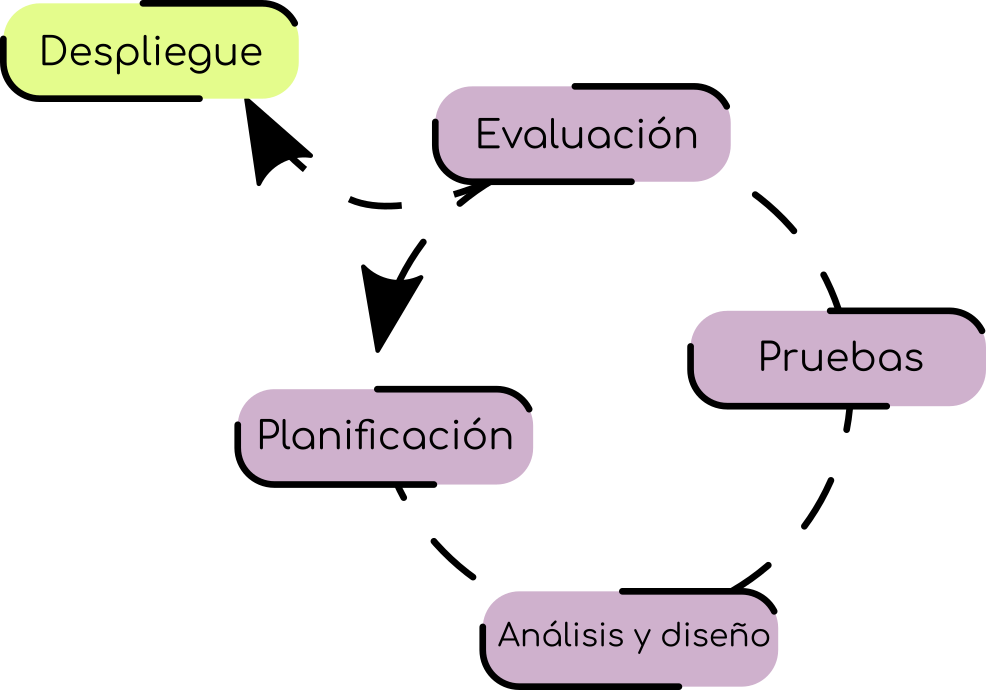
\includegraphics[width=10cm]{figs/desarrollo_iterativo}
  \end{center}
  \caption{Esquema del desarrollo software iterativo.}
  \label{fig:desarrollo_iterativo}
\end{figure}\

Este desarrollo implicó pruebas periódicas en simulación con el fin de
identificar errores y perfeccionar los valores de los parámetros, para
posteriormente evaluar su funcionamiento en un entorno real, concretamente en el
Laboratorio de Robótica del Aulario 3 de la Universidad Rey Juan Carlos.

%Qué paradigma de desarrollo software has seguido para alcanzar tus objetivos.

\section{Plan de trabajo}
\label{sec:plantrabajo}

El desarrollo del proyecto ha comprendido varias etapas, que incluyen la
investigación del \textit{software} a utilizar, la investigación del estado del
arte, la implementación de una arquitectura \textit{software} funcional en los
distintos entornos y el desarrollo del \textit{software} demostrativo o de
ejemplo, comprendiendo un periodo de tiempo superior a un año, comenzando en
febrero de 2023 y finalizando en junio de 2024.

\begin{enumerate}
    \item{\textit{Investigación del software a utilizar.} Periodo de febrero a
        mayo de 2023 durante las prácticas de empresa, en las que estuve
        aprendiendo el funcionamiento de \textit{softwares} como Zenoh,
        Zenoh-Flow, Zenoh-Bridge-DDS, CycloneDDS, y acerca de las
        telecomunicaciones entre robots, 35 horas semanales durante 4 meses.}
    \item{\textit{Investigación del estado del arte.} Periodo de junio a agosto
        de 2023, en el que se investigó acerca de los trabajos previos
        relacionados, y sobre la viabilidad y compatibilidad del proyecto.}
    \item{\textit{Implementación de una arquitectura software funcional en
        simulación.} Periodo de junio a agosto de 2023, en el que se consiguió
        un correcto funcionamiento del \textit{software} en simulación.}
    \item{\textit{Desarrollo de software demostrativo.} Periodo de agosto a
        noviembre de 2023 en el que se migró el \textit{software} desarrollado
        durante las prácticas a versiones posteriores.}
    \item{\textit{Implementación de una arquitectura software funcional en un
        entorno real.} Periodo de noviembre de 2023 a enero de 2024 en el que se
        consiguió un correcto funcionamiento del \textit{software} en el
        laboratorio.}
    \item{\textit{Pruebas del software desarrollado en el laboratorio.} Periodo
        de noviembre de 2023 a abril de 2024 en el que se realizaron las pruebas
        y cambios necesarios para un correcto funcionamiento del
        \textit{software} demostrativo en el entorno real del laboratorio.}
    \item{\textit{Escritura de la memoria.} Periodo de marzo a junio de 2024 en
        el que se elaboró el presente documento, así como la presentación para
        su defensa.}
\end{enumerate}

Durante los periodos de desarrollo de este proyecto fuera de las prácticas de
empresa, se dedicaban aproximadamente de 30 a 40 horas semanales, manteniendo
reuniones con el tutor, que generalmente se llevaban a cabo semanalmente, y
ocasionalmente cada dos semanas.
\\

Todo el proceso de trabajo se ha ido alojando en un repositorio público de
GitHub\footnote{
\href{https://github.com/RoboticsURJC/tfg-unai}{https://github.com/RoboticsURJC/tfg-unai}}.
Asimismo, el trabajo diario se ha ido documentando detalladamente en la
Wiki\footnote{
\href{https://github.com/RoboticsURJC/tfg-unai/wiki}{https://github.com/RoboticsURJC/tfg-unai/wiki}}
de dicho repositorio, haciendo las veces de cuaderno de bitácora, donde quedan
reflejados todos los contratiempos, soluciones y pruebas realizadas.

%Qué agenda has seguido. Si has ido manteniendo reuniones semanales, cumplimentando objetivos parciales, si has ido afinando poco a poco un producto final completo, etc.
